\begin{samplecase}
{\bf Coupled-channels rotational model: n + ${}^{28}$Si}\newline
In this sample case, we consider spherical OMP and rotational coupled-channels
calculations for the deformed nucleus ${}^{28}$Si.
\subsubsection{Case a: Spherical optical model}
In the first case, we treat ${}^{28}$Si as a spherical nucleus and include
the first ($2^{+}$), second ($4^{+}$) and sixth ($3^{-}$) level as weakly
coupled levels, i.e. the cross sections are calculated with DWBA.
The input file is

\VerbatimInput{\samples n-Si028-cc/org/talys.inp}


For the default calculation, TALYS will look in the {\em deformation/exp}
database to see whether a coupling scheme is given. Since this is the case for
${}^{28}$Si, we have to put {\bf spherical y} to enforce a spherical
calculation.
\subsubsection{Case b: Symmetric rotational model}
In the second case,
we include the first and second level of the ground state rotational band
and the $3^{-}$ state in the coupling scheme. This is accomplished with the
input file

\VerbatimInput{\samples n-Si028-cc-sym/org/talys.inp}

In Fig.~\ref{siinel}, the calculated total inelastic scattering for cases a and
b are plotted.
\end{samplecase}
\begin{figure}
\centering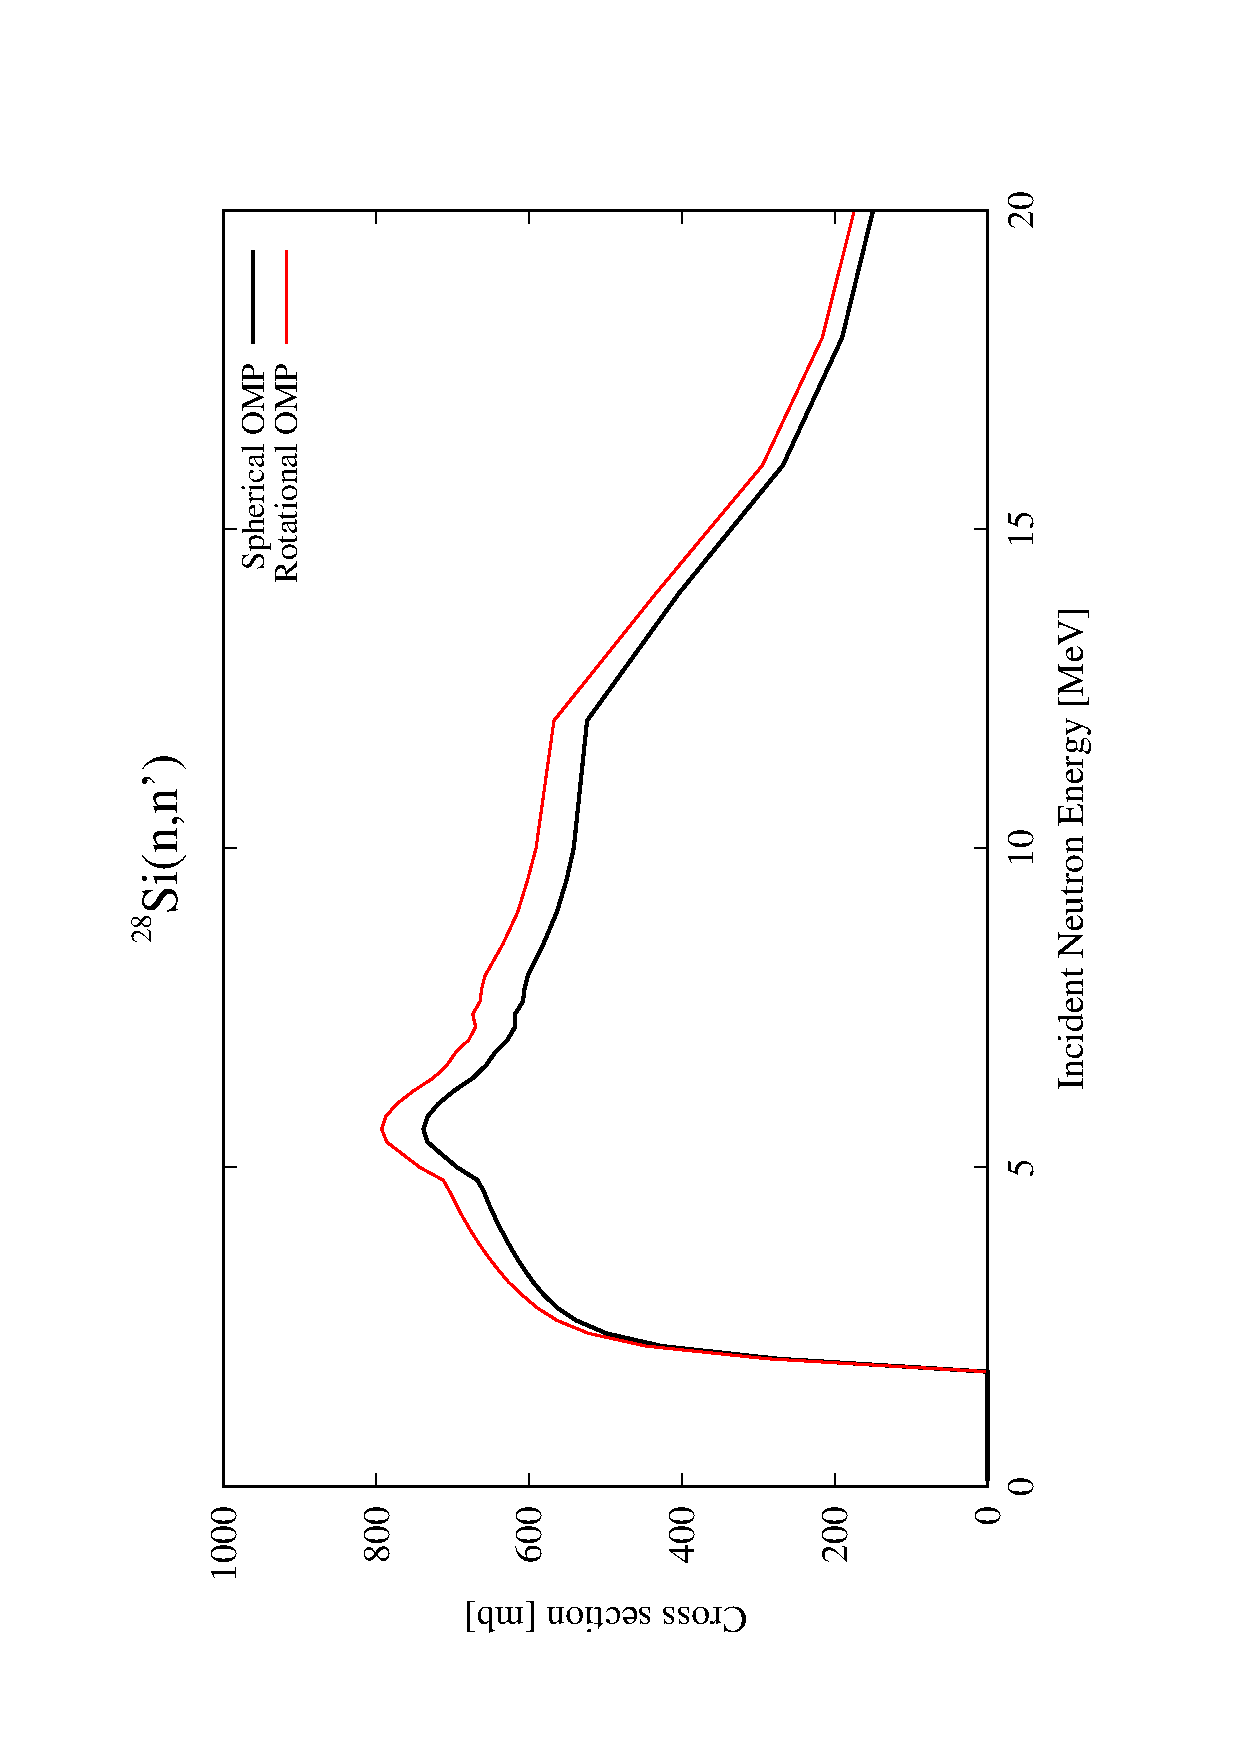
\includegraphics[scale=0.5,angle=270]{n-Si028-inel}
\caption{Total inelastic neutron scattering off ${}^{28}$Si for a spherical
and a deformed OMP.}
\label{siinel}
\end{figure}

